\begin{figure*}[ht]
\centering
 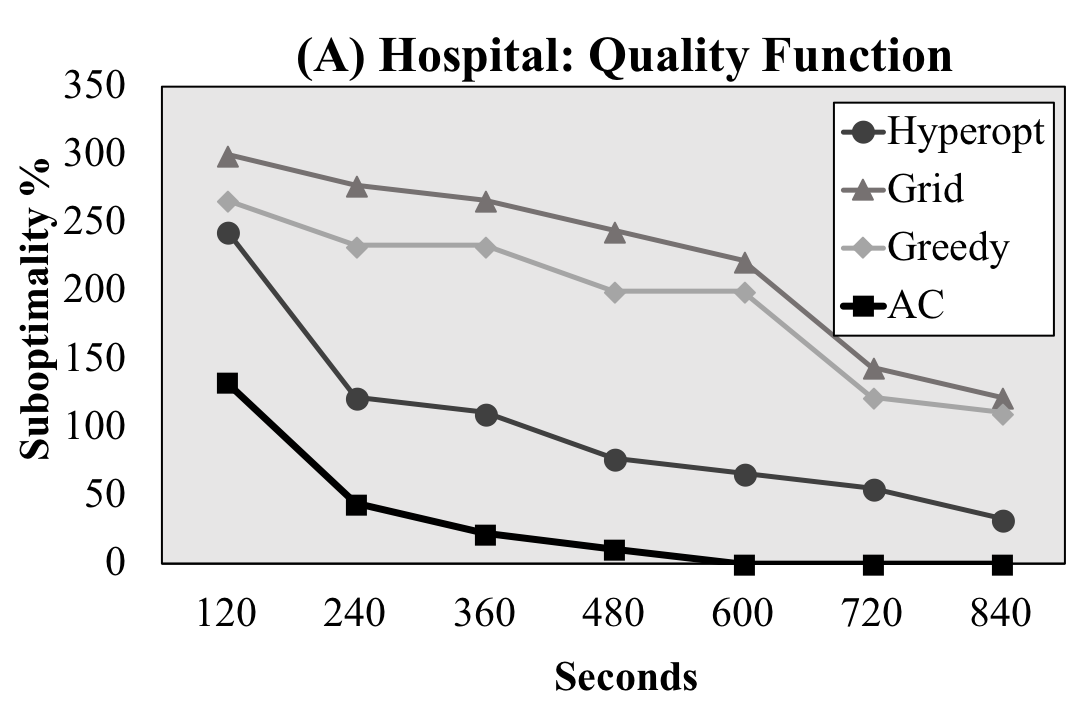
\includegraphics[width=0.32\textwidth]{exp/exp2a.png}
 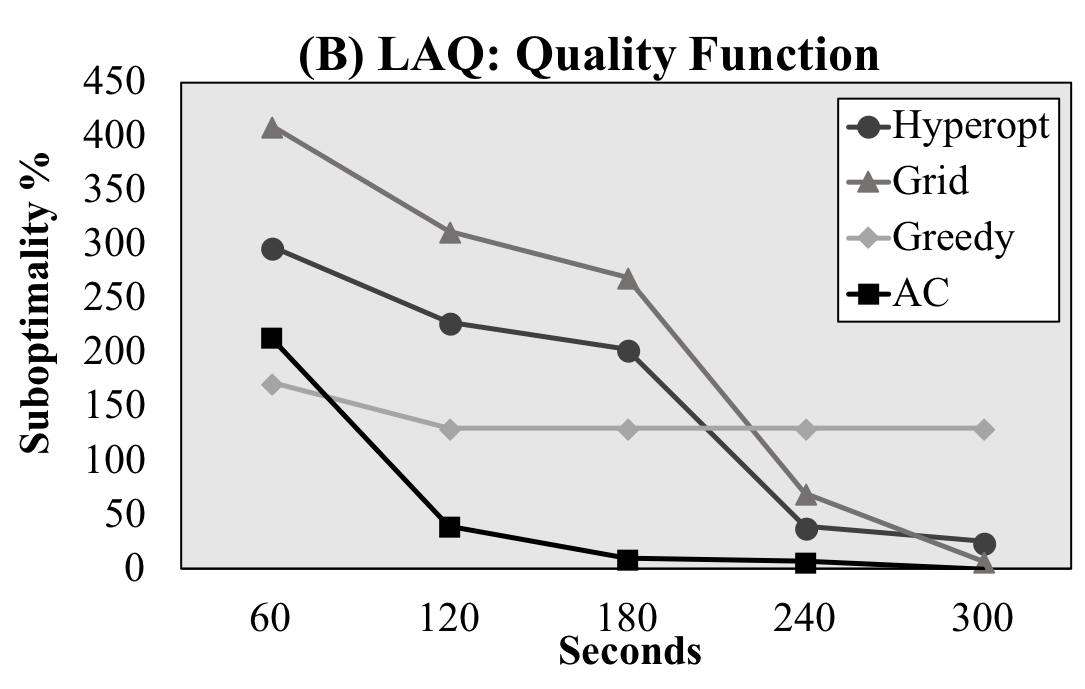
\includegraphics[width=0.32\textwidth]{exp/exp2b.png}
 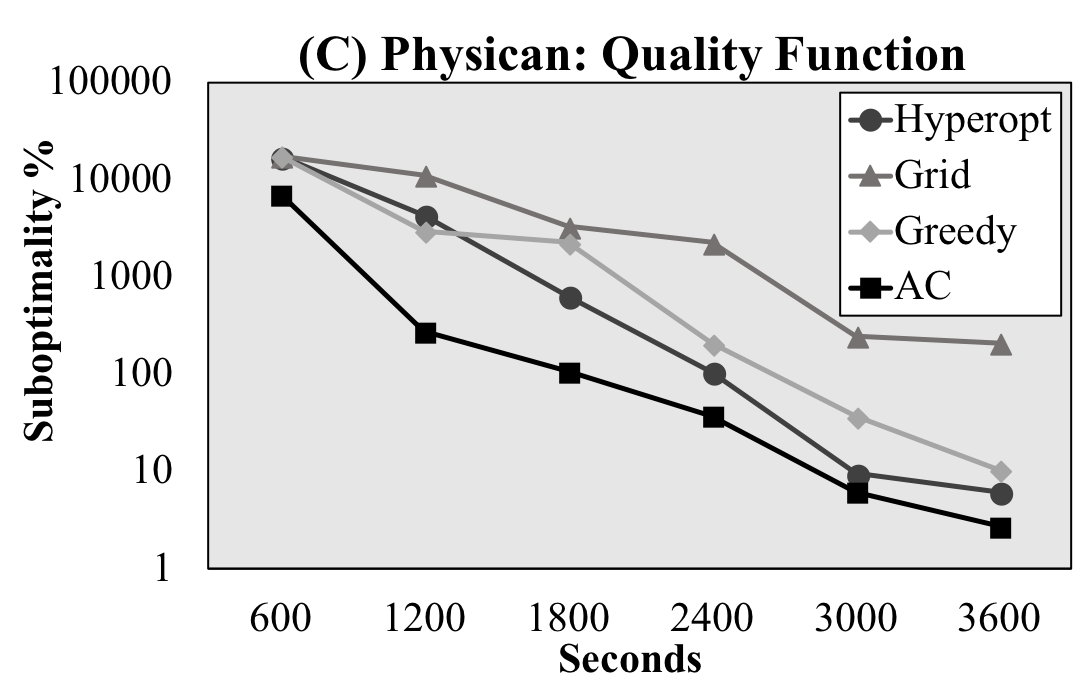
\includegraphics[width=0.32\textwidth]{exp/exp2c.png}
 \caption{ Tuning Against Quality Functions. On the x-axis is the search time in seconds, and on the y-axis is the suboptimality w.r.t the quality of the ground truth data. (A) Hospital dataset, (B) London Air Quality Dataset, (C) Physician Dataset. In all three datasets, \sys converges to a more accurate solution faster than the alternatives. \label{exp2}}
\end{figure*}

\begin{figure*}[ht]
\centering
 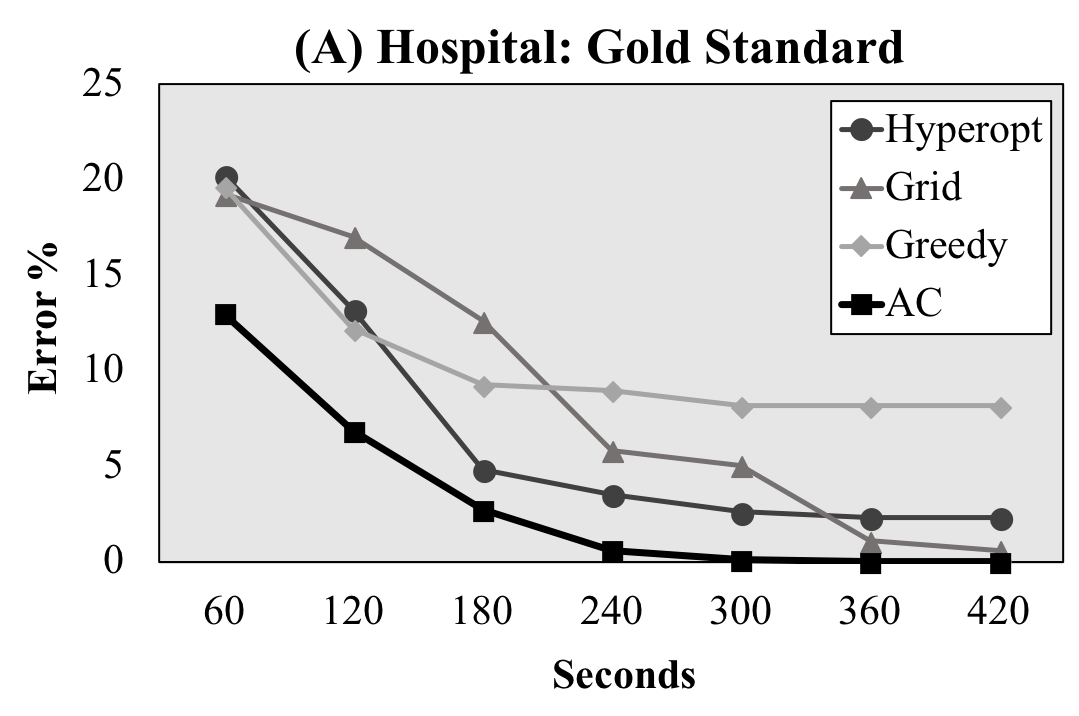
\includegraphics[width=0.32\textwidth]{exp/exp1a.png}
 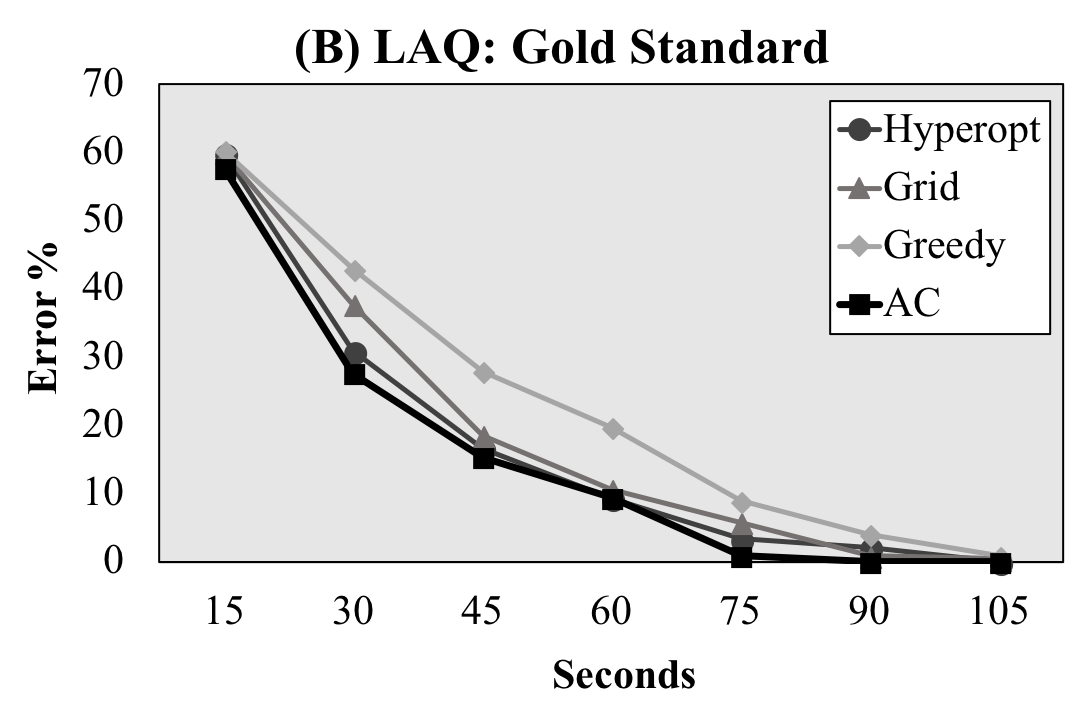
\includegraphics[width=0.32\textwidth]{exp/exp1b.png}
 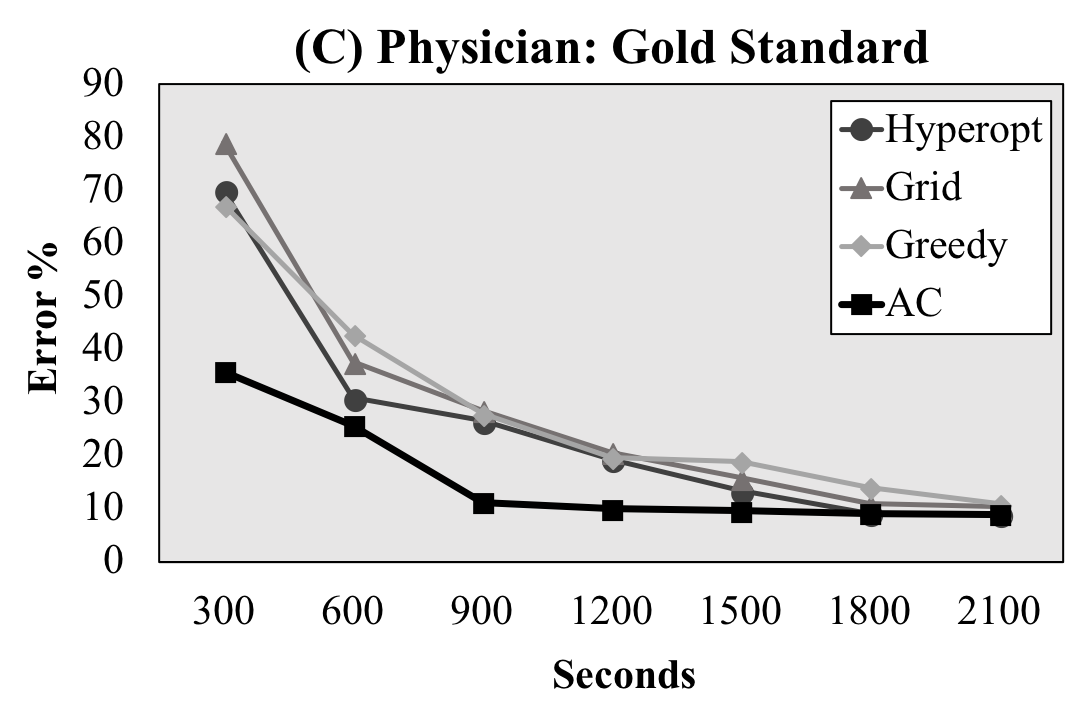
\includegraphics[width=0.32\textwidth]{exp/exp1c.png}
 \caption{ Tuning Against Gold-Standard Data. On the x-axis is the search time in seconds, and on the y-axis is the inaccuracy w.r.t ground truth. (A) Hospital dataset, (B) London Air Quality Dataset, (C) Physician Dataset. In all three datasets, \sys converges to a more accurate solution faster than the alternatives.   \label{exp1}}
\end{figure*}

\section{Experiments}\label{s:exp}
The goal of our experiments is to 1) compare \sys with modern blackbox hyper-parameter tuning algorithms, 2) to understand its strengths and weaknesses, and 3) to highlight the promise of a general search-based method through comparisons with data cleaning systems such as HoloClean~\cite{rekatsinas2017holoclean} that are specialized to specific classes of data errors. 

% We compare \sys to both other hyper-parameter tuning frameworks as well as end-to-end data cleaning systems when applicable. Our results show that: (1) \sys can tune data cleaning pipelines for a large variety of quality functions, (2) the asynchronous architecture in \sys is robust to redundant/slow/incorrect pipeline components, and (3) the optimizations in \sys can improve optimization performance by more than 20x.



\subsection{Datasets and Baselines}
We focus on three datasets used in prior data cleaning benchmarks.  Each dataset exhibits different dataset sizes and data cleaning needs. Each dataset also provides ground truth cleaned versions. We also describe the default cleaning operator libraries for each dataset, informed on prior benchmarks, as well as baseline hyper-parameter tuning methods.

\subsubsection{Datasets and Cleaning Benchmarks}


\stitle{Hospital} This dataset contains UK Hospital information, and used in~\cite{he2016interactive, rekatsinas2017holoclean}.  Roughly 5\% of the cells are corrupted with mispellings, missing values, or other inconsistencies.  The default quality function tries to minimize the number of singleton cities with only one hospital, because it may be due to data errors (example in Section~\ref{s:problem}).  The default library contains: \texttt{ispell.replace(thresh, attr)} as described in Section~\ref{s:problem} replaces the attribute value if it is within a threshold of a dictionary value, \texttt{minhash.replace(thresh, attr)} runs the minhash de-duplication algorithm~\cite{broder2000min} to find similar values and sets them to be equal, and \texttt{fd.replace(fd)} enforces a functional dependency with the chase algorithm~\cite{aho1979theory}.

\stitle{London Air Quality (LAQ)} The dataset contains measurements of air pollution particulate matter from London boroughs~\footnote{\url{https://www.londonair.org.uk/london/asp/datadownload.asp}}. Around 2\% of the measurements (cells) are corrupted by a variety of different outliers including very large values as well as clipped very small values.  As the errors are mostly numerical in this dataset, the default quality function fits an autoregressive model to the windows and computes the average error to the fit model:
\begin{verbatim}
    SELECT AVG(autoregression.error(window))
    FROM data [Range 5 hours];
\end{verbatim}
\noindent The default library consists of parametrized outlier detector methods from dBoost~\cite{mariet2016outlier} and pyod\footnote{\url{https://pyod.readthedocs.io/en/latest/}}.  Both detect outliers and set them to the last known non-outlier value. \texttt{dBoost.histogram(peak\_theshold, outlier\_threshold, window\_size)} detects peaks in histograms of sliding windows of the data, \texttt{dBoost.gaussian(K, window\_size)} thresholds values outside $K$ standard deviations  from the mean of a sliding window, and \texttt{pyod.pca(outlier\_threshold, window\_size)}  applies PCA to sliding windows and thresholds them by the sum of weighted projected distances to the eigenvector hyperplane.

\stitle{Physician} The Physician Compare dataset was used in HoloClean~\cite{rekatsinas2017holoclean}, and contains information on medical professionals and the primary care practice they are associated with.  It contains misspellings, inconsistencies, and missing data. The default quality function is the set of 8 functional dependencies defined in~\cite{rekatsinas2017holoclean}.  The default library contains the operators for the Hospital dataset as well as HoloClean, which is wrapped as the operator (\texttt{holoclean.replace(fd, threshold)}) that enforces a functional dependency using HoloClean's suggested cell value fix if its confidence exceeds a threshold.

\subsubsection{Baselines}
We consider the following baseline techniques by encoding the data cleaning problem into a large set of parameters as described in Section~\ref{s:background}. To speed up the methods, we use the incremental computation optimization for quality function evaluation. Every component is given the same time limit and has to return its best cleaning strategy by that time. 

\stitle{Grid Search} We cascade all of the operators into a fixed order and treat it as a monolithic parametrized unit. We search over all possible values of the discrete parameters and a grid of values over the continuous parameters, and evalute the quality at the end. We use grid search as a baseline as it is easy to parallelize and compare at scale.

\stitle{Hyperopt} We use exactly the same setup as Grid Search but instead of searching over a grid,  we use python hyperopt to perform a Bayesian optimization and intelligently select parameters. We use hyperopt as a baseline for an optimized single-threaded search through the parameter space.

\stitle{Greedy} We tune each data cleaning algorithm independently with respect to the original data. We use a grid search scheme on each component independently. We use greedy as a baseline to illustrate the benefits and drawbacks of individual optimization of each data cleaning system.



\subsection{End-to-End Experiments}
We first compare \sys with the baseline parameter tuning methods on the three benchmark datasets.   For all three benchmarks, we add a component to the quality function that penalizes size of the changes in the cleaned dataset, based on cell-wise edit distance for string values or absolute difference for numeric values.    To understand the  relative convergence of the methods, we report suboptimality, defined as the ratio of the quality score evaluated on the ground truth over the current best quality score.  To understand the absolute cleaning improvements, we report Error, as defined by F1 of current cleaned cells with respect to the ground truth cleaned cells.

Figure \ref{exp2} plots suboptimality convergence over search time in seconds.
All searches are run with one search thread (\sys uses one extra thread to generate conditional assignments across all cleaning operators in a loop).  
We find that \sys quickly finds strong solutions quickly, because the asynchronous design quickly allows for partial data cleaning even if early parameter choices are suboptimal.
Throughout the search process, \sys is up to 9x higher quality than the next best baseline, and ultimately converges to higher quality solutions.  


Figure~\ref{exp1} plots the error rate over search time, but the quality function computes the number of cells that differ from the ground truth dataset.  We consider this the best-case gold standard quality function.
We see that in this case, \sys converges to the ground truth more quickly than the next best baseline (up to $3\times$).


\subsection{Optimization Contributions}

\begin{figure}[t]
\centering
 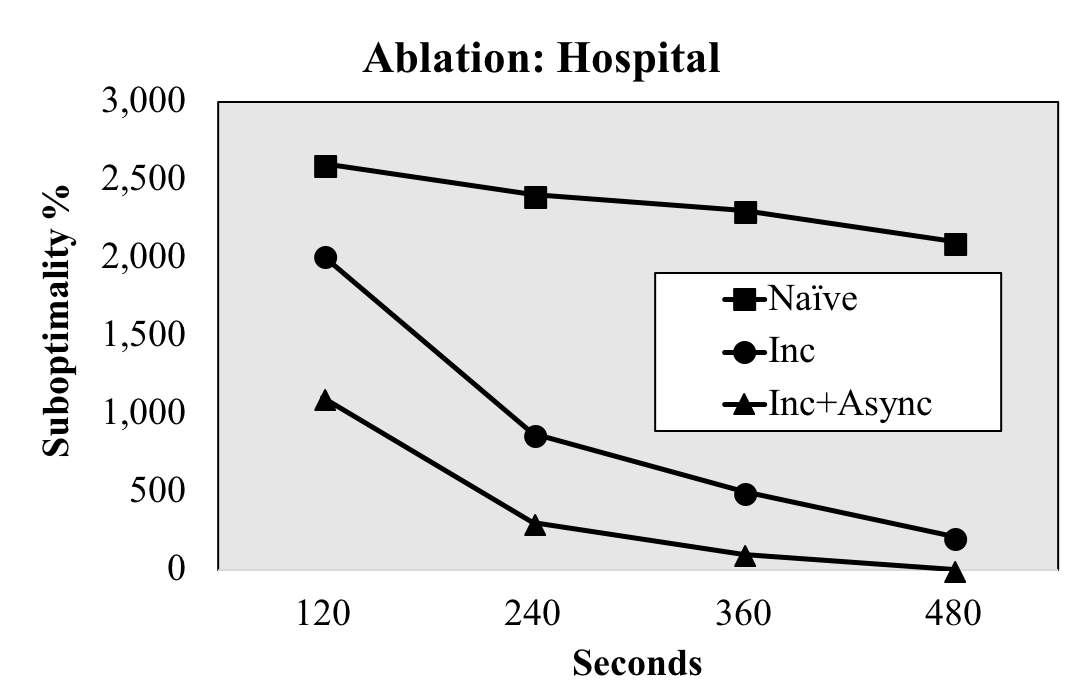
\includegraphics[width=0.8\columnwidth]{exp/exp7a.png}
 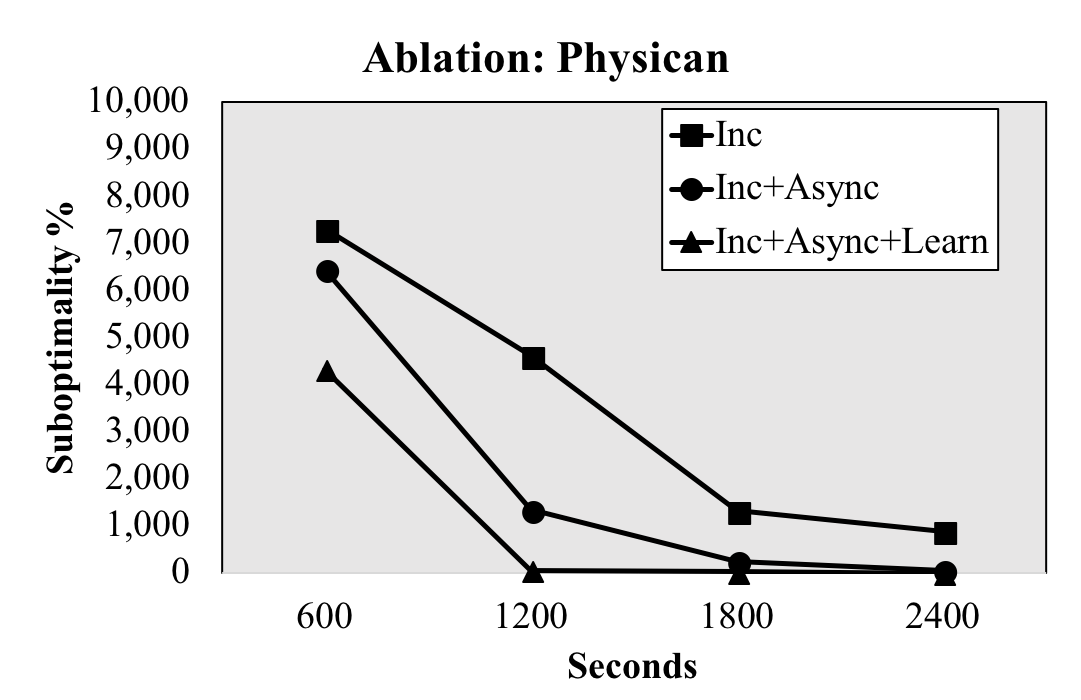
\includegraphics[width=0.8\columnwidth]{exp/exp7b.png}
 \caption{Contribution of the different optimizations. Incremental quality evaluation (Inc), asynchronous search (+Async), and learned pruning models (+Learning) all contribute to improved convergence above Naive. The hospital dataset is too small for learning, and the physician dataset is too large to finish without incremental evaluation. \label{exp7}}
\end{figure}


Figure~\ref{exp7} incrementally removes components of \sys to understand where the benefits come from:  incremental quality evaluation (Inc), asynchronous conditional assignment generation (Async), learning a pruning model (Learn).  We find that \sys without any optimizations (Naive) does not finish on the Physician within an hour due to the large size of the dataset, and that pruning is ineffective for Hospital due to its small size, so do not include them in the plots.

We find that all techniques are crucial.  \sys is designed to quickly evaluate a large number of quality functions, thus Inc is a primary performance optimization. 
Async allows search to quickly explore more pipelines without being blocked by conditional assignment generation, while Learn is able to effectively prune large subsets of the search space when the dataset is large; if the dataset is small there can be too few partitions from which to collect training samples.
These optimizations can improve convergence by more than 20x.



\begin{figure}[t]
\centering
 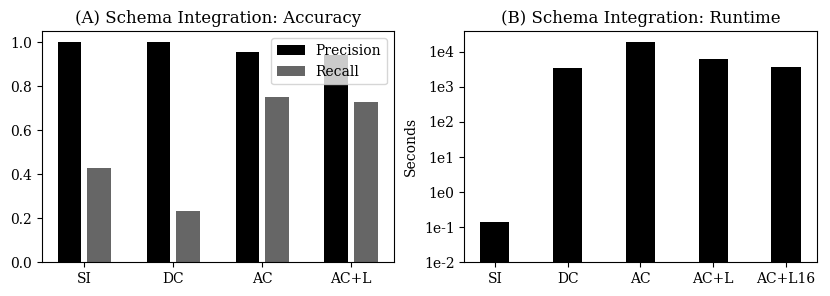
\includegraphics[width=0.8\columnwidth]{exp/exp3.png}
 \caption{Scaling performance on the hospital dataset. \sys can benefit from parallelism. \label{exp3}}
\end{figure}

\subsection{\sys Performance Sensitivity}
We now study settings that affect \sys convergence rates.

\begin{figure}[t]
\centering
 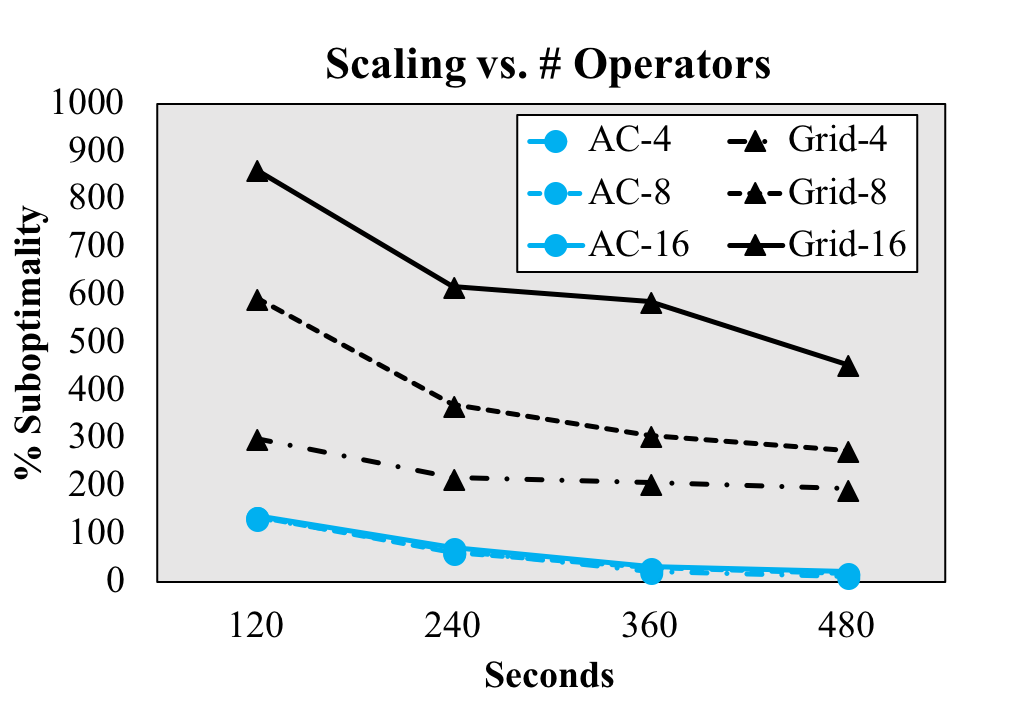
\includegraphics[width=0.8\columnwidth]{exp/exp5.png}
 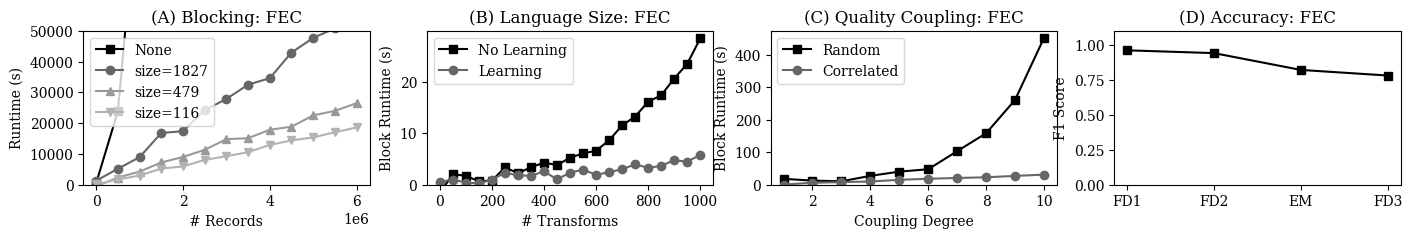
\includegraphics[width=0.8\columnwidth]{exp/exp4.png}
 \caption{Both experiments are on the hospital dataset. (A) Convergence with $4, 8, 16\times$ redundant cleaning operators. (B) Convergence for short $[0-50ms]$ (AC-/HO-) and long $[0-100ms]$ (AC+/HO+) operator delays. \label{exp45}}
\end{figure}

\stitle{Scaling to Cores}
The asynchronous search architecture has desirable scaling properties.
We compare to Grid search and vary the number of threads given to both frameworks.
In \sys, we allocate one thread to each data cleaning method to generate candidate conditional assignments and the remainder to the search algorithm.
Figure \ref{exp3} illustrates the scaling on the hospital dataset.
Results suggest that \sys can benefit from parallelism.

Note that most blackbox approaches such as Grid search can run cleaning operators in parallel, however they block until the operators finish before performing a search step (picking and trying a candidate pipeline) and choosing the next parameters to try.  Thus, they can be blocked by straggler operators.  More sophisticated hyper-parameter tuning algorithms, such as hyperopt are inherently sequential and do not run cleaning operators in parallel.  



\stitle{Library Size} Figure \ref{exp45}b uses the Hospital benchmark and varies the number of redundant cleaning operators, by duplicating the library by $4, 8, 16\times$.  Each duplicate runs in a separate thread.  To exploit parallelism, we compare with grid search (Grid) using the same number of threads.  \sys performs nearly identically irrespective of the redundancy, while grid search degrades considerably due to the reasons described in the above scaling experiment.  


\stitle{Slow Cleaning Operators}
We use the Hospital benchmark to study robustness against slow cleaning operators. Figure \ref{exp45}a compares \sys (AC) to hyperopt (HO) with when adding random delays to the cleaning operators.  Each operator in \sys runs in a separate thread, whereas hyperopt is a sequential algorithm.  \sys is significantly more robust to these delays that hyperopt.

\begin{figure}[h]
\centering
 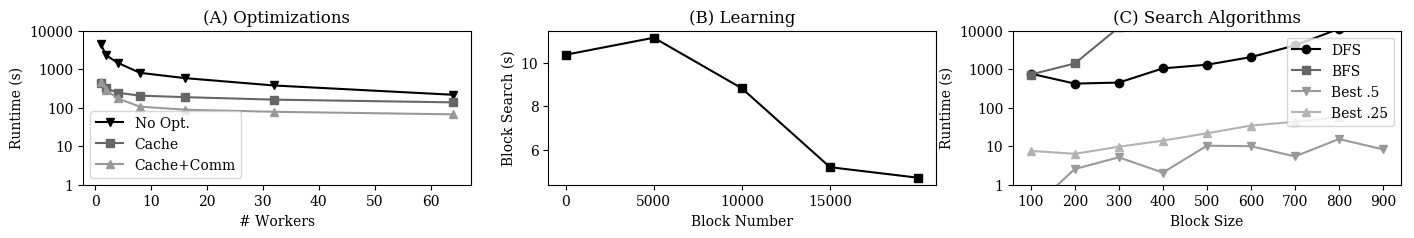
\includegraphics[width=0.8\columnwidth]{exp/exp6.png}
 \caption{Convergence for short $[0-50ms]$ (AC-/HO-) and long $[0-100ms]$ (AC+/HO+) quality function evaluation delays.  \label{exp6}}
\end{figure}


\stitle{Slow Quality Evaluation}
\sys makes a design assumption that the cleaning is the bottleneck and not the quality evaluation. Figure \ref{exp6} runs the Hospital benchmark with varying delays in quality evaluation: AC-/HO- for random $[0-50ms]$ delays, and AC+/HO+ for random $[0-100ms]$ delays. While both \sys (AC) and hyperopt (HO) are affected, \sys is much more sensitive because \sys evaluates quality functions at a far higher rate than hyperopt.




\begin{figure}[h]
\centering
 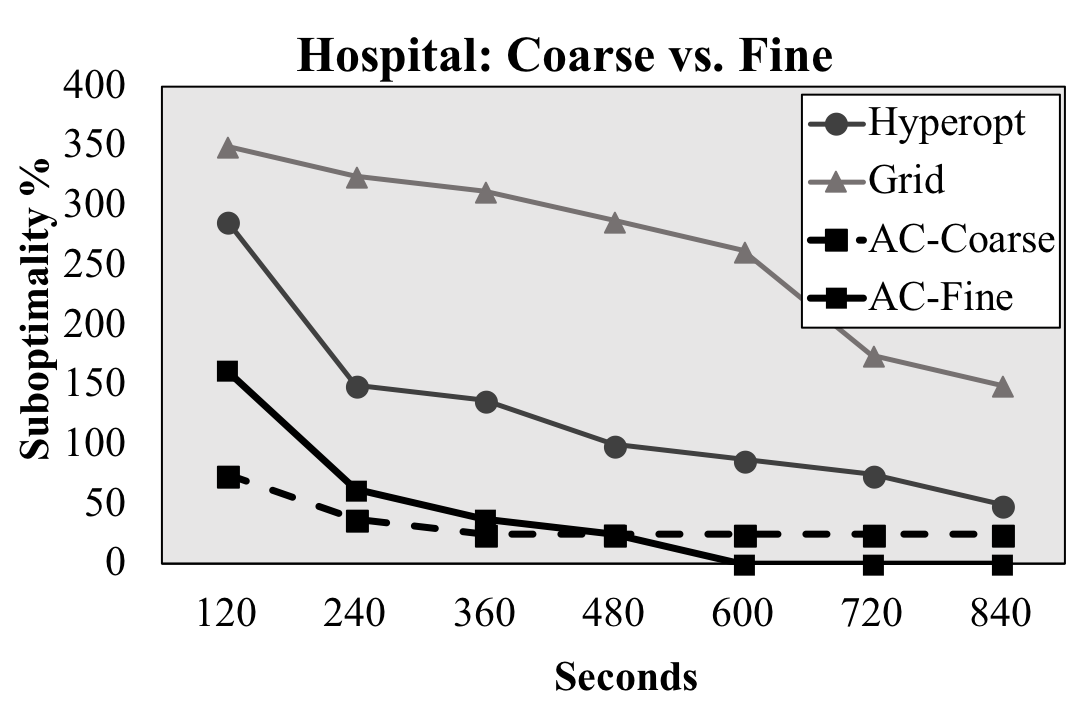
\includegraphics[width=.8\columnwidth]{exp/exp8.png}
 \caption{We apply \sys to the hospital dataset with a coarsed candidate generation scheme. Each data cleaning method produces one full-table transformation per parameter setting (AC-Coarse). While it does not converge to the global solution that the original method does (AC-Fine), it still provides a benefit due to operator exclusion and re-ordering. \label{exp8}}
\end{figure}

\stitle{Coarse vs. Fine Predicates}
Cleaning operators set the predicate granularity of the conditional assignments that they output.  Figure~\ref{exp8} evaluates the trade-off between coarse (AC-Coarse) and fine-grained (AC-Fine) conditional assignment predicates on \sys We generate coarse predicates by merging all conditional assignments generated by an operator into a single ``meta assignment'' that applies the set internally.  The main difference is that \sys cannot pick and choose from within the set.   We see that coarse predicates is initially better because \sys searches through a smaller conditional assignment pool for acceptable pipelines.  However, AC-Fine converges to a better plan because it is capable of making finer-grained decisions later on.  This suggests a potential coarse-then-fine hybrid approach in future work.  We include hyperopt and grid as reference. 




\begin{figure}[h]
\centering
 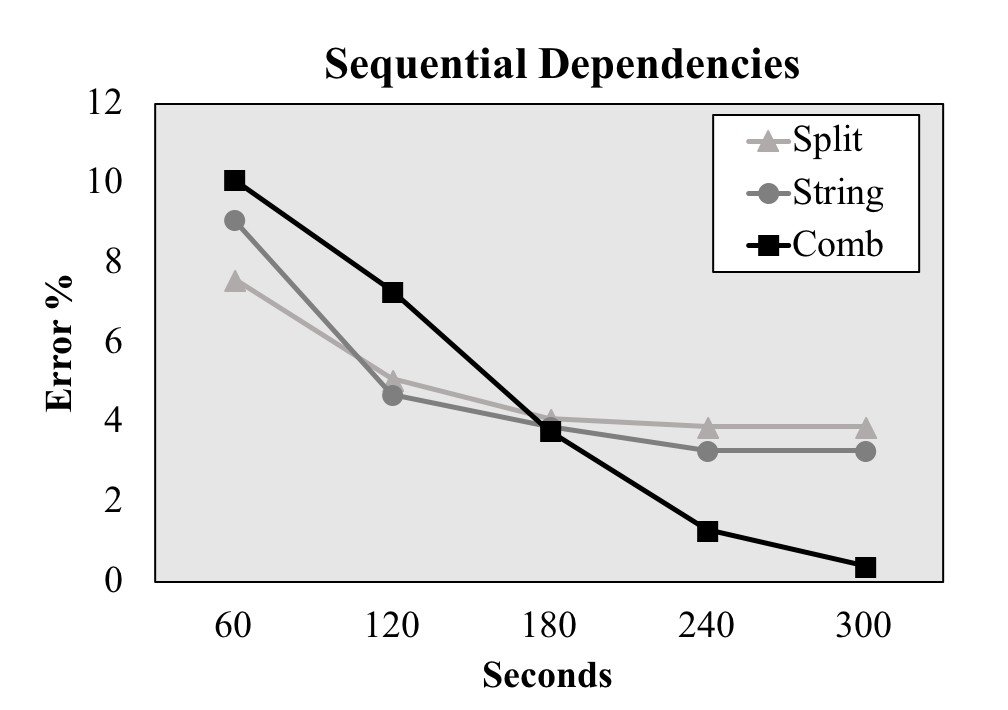
\includegraphics[width=.8\columnwidth]{exp/exp10.png}
 \caption{On a synthetic dataset with extraction and spelling errors, \sys is able to combine two types of cleaning operators (Split, String) in the appropriate sequence to clean the dataset.\label{exp10}}
\end{figure}

\stitle{Sequential Data Cleaning}
It is possible that a best-first search through an asynchronously generated candidate pool may affect problems where the precise sequence of data cleaning operations matters.
In the last experiment, we consider a synthetic dataset similar to the \texttt{City} table in Section~\ref{s:problem}.  
We construct a dataset of 10000 tuples with string attributes \texttt{str1, str2}, and functional dependency \texttt{str1$\rightarrow$str2}.  We pick 5\% of the tuples and add random spelling errors or randomly swapped values. For 50\% of that subset of tuples, we concatenate \texttt{str1:str2} together with a separator drawn from the three characters (\texttt{:,-}).  We then set \texttt{str1} to the resulting string, and \texttt{str2} to `'.  Thus, some tuples need to be correctly split before they can be cleaned to resolve functional dependency violations.

We consider two baseline libraries that each solve one type of error: \texttt{Split} only contains the string split operator, \texttt{String} only contains the string edit operators \texttt{ispell} and \texttt{edit\_dist\_match}.  \texttt{Comb} combines both libraries.  The quality function is the sum of the number of functional dependency violations, spelling errors, and empty strings.  We run \sys with 16 threads.

Figure \ref{exp10} shows that \texttt{Comb} takes longer than the baselines, but is capable of converging to a higher quality over all solutions.
We find that the asynchrony does not affect the sequential dependency and order of operations.
This is because of the tree-search, the operations that improve the quality score will be applied first and those that do not will be ignored.
These ignored operations may later become relevant in later rounds of the algorithm.  It is possible to have degenerate cases that mislead the pruning model, such as if {\it every} tuple must first be split before string edit fixes have any effect.  However, this is unlikely othewise.

{\it \stitle{Takeaways} \sys is designed to explore the plan space by leveraging the structure of data cleaning problems and out-performs generic blackbox parameter tuners.  Evidence suggests that \sys scales across cores, is robust to many forms of delays or redundancies, but is highly sensitive to slow quality evaluation.  Designing a system that adjusts to slow operators or quality evaluations is a promising direction for future work.}

\begin{figure}[h]
\centering
 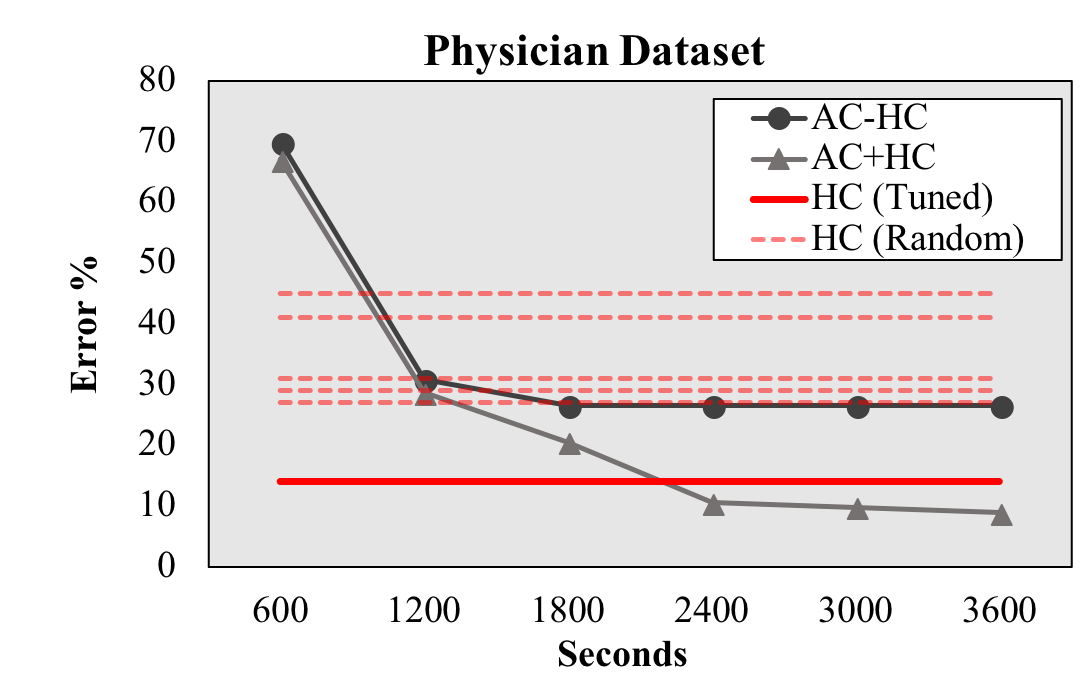
\includegraphics[width=0.7\columnwidth]{exp/exp9a.png}
 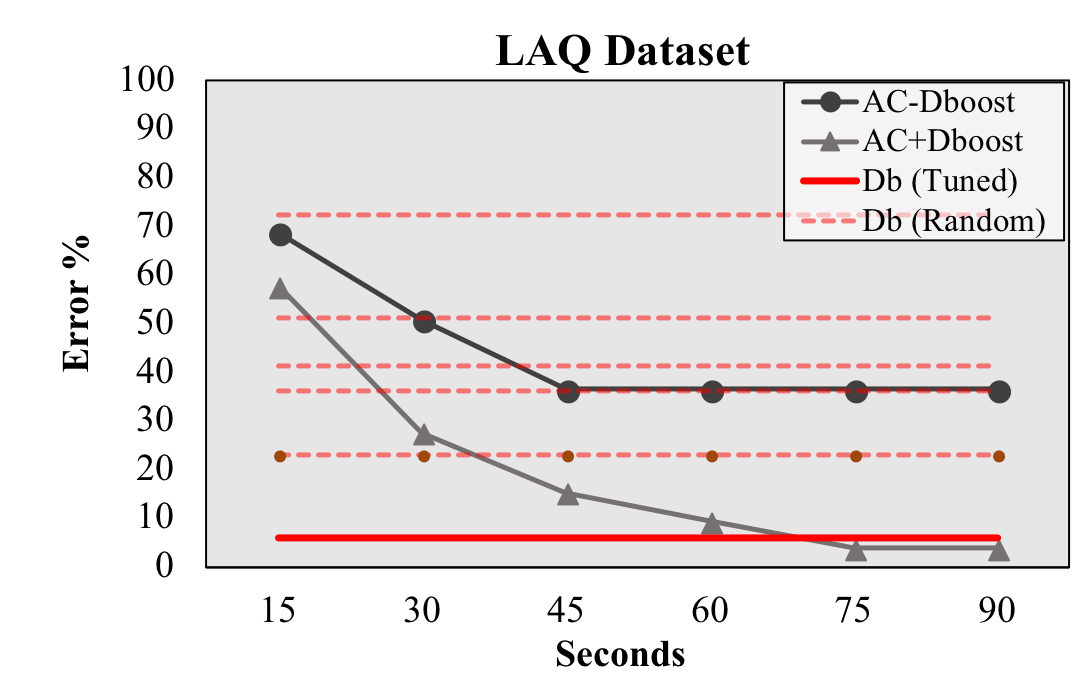
\includegraphics[width=0.7\columnwidth]{exp/exp9b.png}
 \caption{We compare \sys on the physician dataset and the air quality dataset against single standalone systems that address functional dependencies (Holoclean HC) and numerical errors (DBoost) respectively. \sys can support both types of errors and wrap around a variety of frameworks, and tune these frameworks.  Standalone system performance on 5 random parameters is shown as dashed lines.   \label{exp9}}
\end{figure}

\subsection{Comparison w/ Standalone Systems}
We now compare \sys with 2 standalone cleaning systems optimized for specific classes of  errors: HoloClean~\cite{rekatsinas2017holoclean} cleans functional dependency violations in the Physician data and dBoost~\cite{mariet2016outlier} detects numerical errors (we use last known good value as the replacement) in the LAQ data.  We compare \sys with the default library, the standalone system, and \sys with the standalone system wrapped as a cleaning operator. Note that \sys's quality function expresses both benchmarks, whereas each standalone system only expresses one of the two.

Figure \ref{exp9}a-b illustrates the results.
Even when a single data cleaning method can directly optimize the quality specification (i.e., integrity constraints), it might be beneficial to apply \sys to address the weak spots of the method. On the physician dataset, Holoclean (HC) achieves an accuracy of 86\% on its own, \sys without using Holoclean (AC-HC) achieves 73\%, and with using Holoclean (AC+HC) achieves 91\%. Similarly, on the air quality dataset, AC+DBoost achieves the best results and an even higher accuracy that DBoost on its own.
Furthermore, the standalone systems themselves are difficult to tune. 
Figure \ref{exp9}a-b plot the best version we found through manual parameter tuning (\red{solid lines}), as well as 5 runs with randomly sampled parameter values (\red{dashed lines}).  We find that the random parameters are highly unpredictable and often generate far worse results than either \sys variants.

{\it \stitle{Takeaways} \sys can model standalone systems as cleaning operators and improve the quality more than \sys or the standalone system on their own.   }



\iffalse
\subsection{Composing Quality Functions}
In many settings, the user incrementally composes a quality function over time, as she learns more about issues in the dataset or their effects on her application.  In this experiment, we rerun \sys as we add more components $q_i$ to a composite quality function $Q_k = \sum_{i=0}^k q_i$ for up to $k=4$, and we measure the convergence curves for each iteration.
We start with the hospital dataset and consider a set of 4 functional dependencies that determine a single attribute (the city name). We incrementally add each of these dependencies to the quality function--increasingly constraining the problem.
\sys can share information between these problem instances 
We expect that the learned pruning rules and \ewu{ANYTHING ELSE THAT CAN BE SHARED?} accelerates subsequent invocations of \sys.


{\it \stitle{Takeaways} \sys can leverage previously learned pruning models to speed up future search problems over quality functions that have been augmented with new terms, thus accelerating the human-in-the-loop aspect of data cleaning. }
\fi







% For example, on the physician dataset, our quality function is derived from integrity constraints. One of the constituent methods, HoloClean, can in principle, directly optimize for that specification. On this dataset, HoloClean (HC) achieves an accuracy of 86\% on its own. However, we may want to ensemble HoloClean with other methods to address some of the remaining errors Figure~\ref{exp9}. Without using HoloClean (AC-HC), \sys (AC-HC) achieves 73\%. HoloClean is clearly the dominant cleaning method in our previous experiments as the alternative techniques are not as accurate. However, there is still a benefit to ensembling. By combining \sys with HoloClean (AC+HC), this accuracy improves to 91\%.









